
%%%%%%%%%%%%%%%%%%%%%%%%%%%%%%%%%%%%%%%%%%%%%%%%%%%%%%%%%%{
%\documentclass[twoside,11pt]{article}
\documentclass[UTF8]{ctexart}
%%%%% PACKAGES %%%%%%
\usepackage{pgm2016}
\usepackage{amsmath}
\usepackage{algorithm}
\usepackage[noend]{algpseudocode}
\usepackage{subcaption}
\usepackage[english]{babel}	
\usepackage{paralist}	
\usepackage[lowtilde]{url}
\usepackage{fixltx2e}
\usepackage{listings}
\usepackage{color}
\usepackage{hyperref}
\usepackage{mdframed}

%\usepackage{auto-pst-pdf}
\usepackage{pst-all}
\usepackage{pstricks-add}

%%%%% MACROS %%%%%%
\algrenewcommand\Return{\State \algorithmicreturn{} }
\algnewcommand{\LineComment}[1]{\State \(\triangleright\) #1}
\renewcommand{\thesubfigure}{\roman{subfigure}}
\definecolor{codegreen}{rgb}{0,0.6,0}
\definecolor{codegray}{rgb}{0.5,0.5,0.5}
\definecolor{codepurple}{rgb}{0.58,0,0.82}
\definecolor{backcolour}{rgb}{0.95,0.95,0.92}
\lstdefinestyle{mystyle}{
	backgroundcolor=\color{backcolour},  
	commentstyle=\color{codegreen},
	keywordstyle=\color{magenta},
	numberstyle=\tiny\color{codegray},
	stringstyle=\color{codepurple},
	basicstyle=\footnotesize,
	breakatwhitespace=false,        
	breaklines=true,                
	captionpos=b,                    
	keepspaces=true,                
	numbers=left,                    
	numbersep=5pt,                  
	showspaces=false,                
	showstringspaces=false,
	showtabs=false,                  
	tabsize=2
}
\lstset{style=mystyle}

\newenvironment{problem}[2][问题]
{\begin{mdframed}[backgroundcolor=gray!20] \textbf{#1 #2} \\}
	{\end{mdframed}}

\newenvironment{dingyi}[2][定义]
{\begin{mdframed}[backgroundcolor=gray!20] \textbf{#1 #2} \\}
	{\end{mdframed}}

\newenvironment{dingli}[2][定理]
{\begin{mdframed}[backgroundcolor=gray!20] \textbf{#1 #2} \\}
	{\end{mdframed}}

%%%%%%%%%%%%%%%%%%%%%%%%%%%%%%%%%%%%%%%%%%%%%%%%%%%%%%%%%% 


%%%%%%%%%%%%%%%%%%%%Information%%%%%%%%%%%%%%%%%%%%%%%%%%%
\newcommand\course{sd03431280}
\newcommand\courseName{数值计算方法}
\newcommand\semester{2020·春季}
\newcommand\assignmentNumber{2}
\newcommand\studentName{陈路}
\newcommand\studentEmail{chenlu.scien@gmail.com}
\newcommand\studentNumber{201800301206}
\newcommand\addr{泰山学堂2018级计算机取向}
%%%%%%%%%%%%%%%%%%%%%%%%%%%%%%%%%%%%%%%%%%%%%%%%%%%%%%%%%%



%%%%%%%%%%%%%%%%%%%%%%%%%%%%%%%%%%%%%%%%%%%%%%%%%%%%%%%%%%
    \ShortHeadings{山东大学\quad \semester\quad  \course\quad \courseName}{\addr \quad \studentName \quad \studentNumber}
    \firstpageno{1}
    
    \begin{document}
    
    \title{第\assignmentNumber 章\quad 非线性方程求根}
    
    \author{\name \studentName \email \studentEmail \\
    \studentNumber
    }
    
    \maketitle
%%%%%%%%%%%%%%%%%%%%%%%%%%%%%%%%%%%%%%%%%%%%%%%%%%%%%%%%%%
本文首先简要总结非线性方程求根的相关知识,包括非线性方程求根的基本概念和常见算法及其收敛速率。进而对一些常用算法进行编程实现,并应用到实际问题体会不同算法的优劣性。

\section{非线性方程求根知识总结}
\subsection{不动点迭代法}
\subsubsection{迭代}
迭代是指重复执行一个计算过程,直到找到答案. 首先需要一个函数$g(x)$和起始点$p_{0}$,然后依据迭代规则$p_{k+1}=g(p_{k})$可得到迭代序列$\left\{p_{k}\right\}$. 如果这一序列中的数趋向于某个极限,那么就达到了我们的求解目的.

\subsubsection{不动点迭代}
\begin{dingyi}{1}
	函数$g(x)$的一个\textbf{不动点}是指一个实数$P$,满足$P=g(P)$.
\end{dingyi}

\begin{dingyi}{2}
	迭代$p_{n+1}=g(p_{n})$,其中$n=0,1,\cdots$,称为\textbf{不动点迭代}.
\end{dingyi}

\begin{dingli}{1}
	设$g$是一个连续函数,且$\left\{p_{n}\right\}_{n=0}^{\infty}$是由不动点迭代生成的序列.\\
	如果$\lim _{n \rightarrow \infty} p_{n}=P$,则$P$是$g(x)$的不动点.
\end{dingli}

\textbf{不动点存在性定理}
\begin{dingli}{2}
	设函数$g \in C[a,b]$.\\
	如果对于所有$x \in [a,b]$,映射$y=g(x)$的范围满足$y \in [a,b]$,那么函数$g$在$[a,b]$内至少有一个不动点.\\
	此外,设$g'(x)$定义在$(a,b)$内,且对于所有$x \in (a,b)$,存在常数$0<K<1$使得$|g'(x)| \leqslant K <1$,则函数$g$在$[a,b]$内有唯一的不动点.
\end{dingli}

\textbf{不动点迭代收敛条件}
\begin{dingli}{3}
	设有(i)$g,g'\in C[a,b]$,(ii)$K$是一个大于0的常数,(iii)$p_{0} \in (a,b)$,(iv)对于所有$x \in [a,b]$,有$g(x) \in [a,b]$.\\
	如果对于所有$x \in [a,b]$,有$|g'(x)| \leqslant K < 1$,那么对于任意初始值$p_{0}$, 迭代$p_{n}=g(p_{n-1})$将收敛到唯一的不动点$P \in [a,b]$.
\end{dingli}


设函数$g$满足定理3中的所有条件,当用$p_{n}$去近似$P$时,引入的\textbf{误差边界}为:
\begin{align}
	\left|P-p_{n}\right| \leqslant K^{n}\left|P-p_{0}\right| \text { 对于所有 } n \geqslant 1
\end{align}
\qquad 且
\begin{align}
	\left|P-p_{n}\right| \leqslant \frac{K^{n}\left|p_{1}-p_{0}\right|}{1-K} \text { 对于所有 } n \geqslant 1
\end{align}

\subsection{全局收敛法}
对于任意函数$f(x)=0$,全局收敛法依赖于初始区间$[a,b]$,满足输入函数值$f(a), f(b)$的符号相反. 一旦给定了这个区间,无论区间多大,通过迭代总能找到输入函数一个根.
然而,如果函数$f(x)=0$在区间$[a,b]$上有多个根,则必须使用不同的起始区间寻找每个根.

\subsubsection{二分法}
假设函数$f(x)$在区间$[a,b]$上连续且两端点处函数值$f(a), f(b)$符号相反.
二分法判定过程的第一步是选择中点$c=(a+b)/2$,然后分析可能存在的3种情况:
\begin{enumerate}
	\item 如果$f(a)$和$f(c)$符号相反,则在区间$[a,c]$内存在零点;
	\item 如果$f(c)$和$f(b)$符号相反,则在区间$[c,b]$内存在零点;
	\item 如果$f(c)=0$,则$c$是零点
\end{enumerate}

\begin{dingli}{1}
	设$f \in C(a,b)$,且存在数$r \in [a,b]$满足$f(r)=0$.\\
	如果$f(a)$和$f(b)$的符号相反,且$\left\{c_{n}\right\}_{n=0}^{\infty}$表示二分法生成的中点序列,则
	\begin{align}
		\left|r-c_{n}\right| \leqslant \frac{b-a}{2^{n+1}} \quad \text { 其中 } n=0,1, \cdots
	\end{align}
\end{dingli}

\subsubsection{试位法}
由于二分法的收敛速度较慢,因此试位法对它进行了改进. 假设函数$f(x)$在区间$[a,b]$上连续且两端点处函数值$f(a), f(b)$符号相反. 
二分法使用区间中点进行迭代,如果找到经过点$(a,f(a))$和$(b,f(b))$的割线$L$与$x$轴的交点$(c,0)$,就可以得到一个更好的近似值,即:
\begin{align}
	c=b-\frac{f(b)(b-a)}{f(b)-f(a)}
\end{align}
类似地,会出现3中可能性:
\begin{enumerate}
	\item 如果$f(a)$和$f(c)$符号相反,则在区间$[a,c]$内存在零点;
	\item 如果$f(c)$和$f(b)$符号相反,则在区间$[c,b]$内存在零点;
	\item 如果$f(c)=0$,则$c$是零点
\end{enumerate}

\subsection{局部收敛法}
对于任意函数$f(x)=0$,局部收敛法要求给定一个接近根的近似值以保证收敛性.
局部收敛法的速度远大于全局收敛法的速度. 
一些混合方法首先采用全局收敛法,当迭代逼近根后切换到局部收敛法.

\subsubsection{牛顿法}

\begin{dingli}{1}
	设$f \in C^{2}[a,b]$,且存在数$p \in [a,b]$,满足$f(p)=0$. 如果$f'(p) \neq 0$,则存在一个数$\delta > 0$,对任意初始近似值$p_{0} \in [p-\delta,p+\delta]$,使得由如下迭代定义的序列$\left\{p_{k}\right\}_{k=0}^{\infty}$收敛到$p$:
	\begin{align}
		p_{k}=g\left(p_{k-1}\right)=p_{k-1}-\frac{f\left(p_{k-1}\right)}{f^{\prime}\left(p_{k-1}\right)} \quad \text { 其中 } k=1,2, \cdots
	\end{align}
	其中,函数$g(x)$定义如下:
	\begin{align}
		g(x)=x-\frac{f(x)}{f^{\prime}(x)}
	\end{align}
	并被称为\textbf{牛顿-拉夫森迭代函数}.
\end{dingli}

\subsubsection{割线法}
牛顿法中每次迭代需要计算两个函数:$f(p_{k-1})$和$f'(p_{k-1})$,当函数形式非常复杂时,求其导数往往较为费时,因此需要一种和牛顿法收敛速度一样快且无需计算导数的方法,这就是割线法.
割线法包含的公式与试位法公式一致,只是在关于如何定义每个后续项的逻辑判定上不一样.
割线法需要两个靠近零点$(p,0)$的初始点$(p_{0},f(p_{0}))$和$(p_{1},f(p_{1}))$,定义$p_{2}$为经过两个初始点的直线与x轴的交点的横坐标,即
\begin{align}
	p_{2}=g\left(p_{1}, p_{0}\right)=p_{1}-\frac{f\left(p_{1}\right)\left(p_{1}-p_{0}\right)}{f\left(p_{1}\right)-f\left(p_{0}\right)}
\end{align}
根据两点迭代公式可以得到一般项为:
\begin{align}
	p_{k+1}=g\left(p_{k}, p_{k-1}\right)=p_{k}-\frac{f\left(p_{k}\right)\left(p_{k}-p_{k-1}\right)}{f\left(p_{k}\right)-f\left(p_{k-1}\right)}
\end{align}

\section{分析讨论题}


\begin{problem}{1}
求方程$2 x^{2}+x-15=0$的正根$x*=2.5$近似值,分别利用如下三种格式编程计算:
\begin{enumerate}
	\item $x_{k+1}=15-2x_{k}^{2}, k=0,1,2, \cdots$,取初始值$x_{0}=2$.
	\item $x_{k+1}=\frac{15}{2 x_{k}+1}, k=0,1,2, \cdots$,取初始值$x_{0}=2$.
	\item $x_{k+1}=x_{k}-\frac{2 x_{k}^{2}+x_{k}-15}{4 x_{k}+1}, k=0,1,2, \cdots$,取初始值$x_{0}=2$.
\end{enumerate}
依次计算$x_{1},x_{2}, \cdots,x_{k}, \cdots$,并作图观察解的稳定性、收敛性,并分析原因.
\end{problem}
\textbf{解}:\\
不动点迭代算法的代码实现:
\begin{lstlisting}[language=matlab]
function [k, p, err, P] = fixpt(g, p0, TOL, N)
% Fixed Point Interation
% Input - g    the iteration function as a string
%       - p0   initial guess for the fixed point
%       - TOL  tolerance
%       - N    the maximum number of iterations
% Output - k   the number of iterations carried out
%        - p   the approximation of the fixed point
%        - err the error in the approximation
%        - P   sequence {p_n}

% Initialization
P(1) = p0; % initial guess
if nargin < 3
	TOL = 1e-3; % tolerance default
end
if nargin < 4
	N = 200; % maximum interation default
end

% Compute fixed point
for k = 2:N
	P(k) = feval(g, P(k-1));
	err = abs(P(k) - P(k-1));
	relerr = err/(abs(P(k)) + eps);
	p = P(k);
	fprintf('Interation NO.%d,\t approximation p=%f,\t absolute error=%f,\t relative error=%f\n',...
		k, p, err, relerr);
	if (err < TOL) || (relerr < TOL)
		break, end
end

if k == N
	disp('Maximum number of iterations exceeded');
end
P = P'; % transpose the vector
end
\end{lstlisting}
\textbf{1}. 使用格式“$x_{k+1}=15-2x_{k}^{2}, k=0,1,2, \cdots$,初始值$x_{0}=2$,精确度=$10^{-4}$”时,迭代过程及误差如表\ref{t1}.
\begin{table}[]
	\centering
	\caption{问题1.1迭代过程}
	\label{t1}
	\begin{tabular}{llll}
		\hline
		\multicolumn{1}{c}{\textbf{迭代次数}} & \multicolumn{1}{c}{\textbf{根的估计值}} & \multicolumn{1}{c}{\textbf{误差}} & \multicolumn{1}{c}{\textbf{相对误差}} \\ \hline
		2                                 & 7.000000                           & 5.000000                        & 0.714286                          \\ \hline
		3                                 & -83.000000                         & 90.000000                       & 1.084337                          \\ \hline
		4                                 & -13763.000000                      & 13680.000000                    & 0.993969                          \\ \hline
		5                                 & -378840323.000000                  & 378826560.000000                & 0.999964                          \\ \hline
		6                                 & -287039980661488672.000000         & 287039980282648352.000000       & 1.000000                          \\ \hline                         
	\end{tabular}
\end{table}
在此情况下,算法无法收敛.\\
\textbf{2}. 使用格式“$x_{k+1}=\frac{15}{2 x_{k}+1}, k=0,1,2, \cdots$,初始值$x_{0}=2$”时,迭代过程及误差如表\ref{t2}.\\
\begin{table}[]
	\centering
	\caption{问题1.2迭代过程(部分省略)}
	\label{t2}
	\begin{tabular}{llll}
		\hline
		\multicolumn{1}{c}{\textbf{迭代次数}} & \multicolumn{1}{c}{\textbf{根的估计值}} & \multicolumn{1}{c}{\textbf{误差}} & \multicolumn{1}{c}{\textbf{相对误差}} \\ \hline
		2                                 & 3.000000                           & 1.000000                        & 0.333333                          \\ \hline
		3                                 & 2.142857                           & 0.857143                        & 0.400000                          \\ \hline
		4                                 & 2.837838                           & 0.694981                        & 0.244898                          \\ \hline
		5                                 & 2.246964                           & 0.590874                        & 0.262966                          \\ \hline
		6                                 & 2.730287                           & 0.483324                        & 0.177023                          \\ \hline
		7                                 & 2.321775                           & 0.408513                        & 0.175948                          \\ \hline
		8                                 & 2.657902                           & 0.336127                        & 0.126463                          \\ \hline
		9                                 & 2.374995                           & 0.282907                        & 0.119119                          \\ \hline
		10                                & 2.608700                           & 0.233706                        & 0.089587                          \\ \hline
		$\cdots$                          & $\cdots$                           & $\cdots$                        & $\cdots$                          \\ \hline
		20                                & 2.517270                           & 0.037851                        & 0.015036                          \\ \hline
		21                                & 2.485691                           & 0.031578                        & 0.012704                          \\ \hline
		22                                & 2.511981                           & 0.026290                        & 0.010466                          \\ \hline
		23                                & 2.490055                           & 0.021926                        & 0.008805                          \\ \hline
		24                                & 2.508315                           & 0.018259                        & 0.007280                          \\ \hline
		25                                & 2.493090                           & 0.015225                        & 0.006107                          \\ \hline
		26                                & 2.505771                           & 0.012681                        & 0.005061                          \\ \hline
		27                                & 2.495200                           & 0.010572                        & 0.004237                          \\ \hline
		28                                & 2.504007                           & 0.008807                        & 0.003517                          \\ \hline
		29                                & 2.496666                           & 0.007341                        & 0.002940                          \\ \hline
		30                                & 2.502782                           & 0.006116                        & 0.002444                          \\ \hline
		$\cdots$                          & $\cdots$                           & $\cdots$                        & $\cdots$                          \\ \hline
		40                                & 2.500449                           & 0.000988                        & 0.000395                          \\ \hline
		41                                & 2.499626                           & 0.000823                        & 0.000329                          \\ \hline
		42                                & 2.500312                           & 0.000686                        & 0.000274                          \\ \hline
		43                                & 2.499740                           & 0.000572                        & 0.000229                          \\ \hline
		44                                & 2.500217                           & 0.000476                        & 0.000191                          \\ \hline
		45                                & 2.499820                           & 0.000397                        & 0.000159                          \\ \hline
		46                                & 2.500150                           & 0.000331                        & 0.000132                          \\ \hline
		47                                & 2.499875                           & 0.000276                        & 0.000110                          \\ \hline
		48                                & 2.500104                           & 0.000230                        & 0.000092                          \\ \hline
	\end{tabular}
\end{table}
在此情况下,算法经过48次迭代后达到精度$10^{-4}$,根的估计值为2.500104.\\
迭代过程可以通过图\ref{fig:figure1}可视化呈现.\\
\begin{figure}[H]
	\begin{center}
		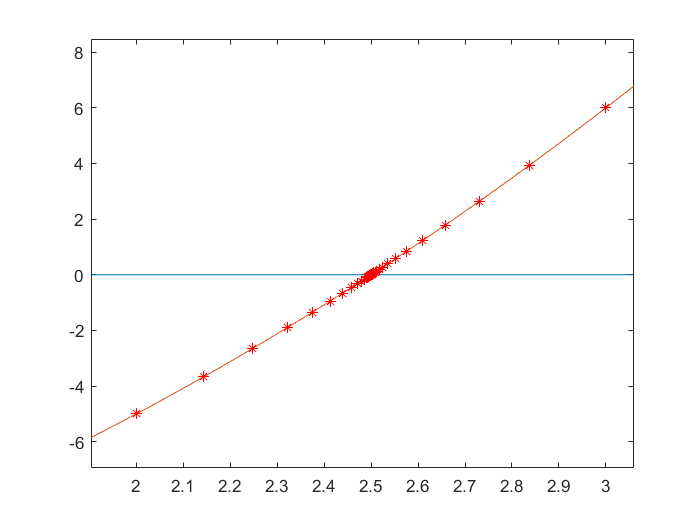
\includegraphics[width=0.7\columnwidth]{figures/problem2.png}
		\caption{问题1.2的迭代过程图示}
		\label{fig:figure1}
	\end{center}
\end{figure}
\textbf{3}. 使用格式“$x_{k+1}=x_{k}-\frac{2 x_{k}^{2}+x_{k}-15}{4 x_{k}+1}, k=0,1,2, \cdots$,初始值$x_{0}=2$”时,迭代过程及误差如表\ref{t3}
\begin{table}[]
	\centering
	\caption{问题1.3迭代过程}
	\label{t3}
	\begin{tabular}{llll}
		\hline
		\multicolumn{1}{c}{\textbf{迭代次数}} & \multicolumn{1}{c}{\textbf{根的估计值}} & \multicolumn{1}{c}{\textbf{误差}} & \multicolumn{1}{c}{\textbf{相对误差}} \\ \hline
		2                                 & 2.555556                           & 0.555556                        & 0.217391                          \\ \hline
		3                                 & 2.500550                           & 0.055006                        & 0.021997                          \\ \hline
		4                                 & 2.500000                           & 0.000550                        & 0.000220                          \\ \hline
		5                                 & 2.500000                           & 0.000000                        & 0.000000                          \\ \hline
	\end{tabular}
\end{table}
在此情况下,算法经过5次迭代后达到精度$10^{-4}$,根的估计值为2.500000.\\
迭代过程可以通过图\ref{fig:figure2}可视化呈现.
\begin{figure}[H]
	\begin{center}
		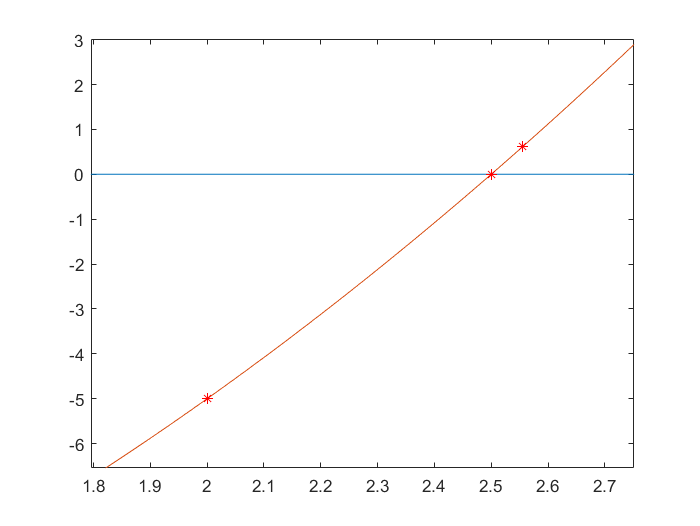
\includegraphics[width=0.7\columnwidth]{figures/problem3.png}
		\caption{问题1.3的迭代过程图示}
		\label{fig:figure2}
	\end{center}
\end{figure}

\begin{problem}{2}
	证明方程$2-3 x-\sin (x)=0$在$(0,1)$内有且仅有一个实根,使用二分法求误差不大于$0.0005$的根及其需要迭代的次数.
\end{problem}
\textbf{解}:\\
令$f(x)=2-3x-sin(x)$,则$f'(x)=-3-cos(x)<0$,所以$f(x)$在区间(0,1)内单调递减. \\
又因为$f(0)=2>0,f(1)=-1-sin1<0$,所以$f(x)$在$(0,1)$内有且仅有一个实根.\\
二分法的代码实现:
\begin{lstlisting}[language=matlab]
function [c, yc, err] = bisect(f, a, b, TOL)
% Bisection method
% Input - f   the input function as a string
%       - a   the left end point of the initial section
%       - b   the right end point of the initial section
%       - TOL tolerance
% Output - c   the zero point of input function
%        - yc  = f(c)
%        - err the error in the approximation

% Initialization
ya = feval(f, a);
yb = feval(f, b);
% Check condition
if ya*yb > 0
	disp('The end-points value of the initial section should not be of the same sign');
return
end

% Compute the number of needed iteration round
N = 1 + round((log(b-a)-log(TOL))/log(2));
% Main process
for k = 1:N
	c = (a+b)/2;
	yc = feval(f, c);

	% Print intermediate messages
	fprintf('Interation NO.%d,\t current section = [%f,%f],\t c=%f,\t f(c)=%f\n',...
		k, a, b, c, yc);

	if yc == 0
		a = c;
		b = c;
	elseif yb * yc > 0
		b = c;
		yb = yc;
	else
		a = c;
		ya = yc;
	end

	if (b - a) < TOL
		break, end
	end

	c = (a + b)/2;
	yc = feval(f, c);
	err = abs(b-a);
end
end
\end{lstlisting}\label{bisect}
经过11次迭代后误差为$-2.454600314258926\times 10^{-4}$.\\
此时根c= 0.505371093750000\\


\begin{problem}{3}
	利用牛顿法求解方程
	\begin{align}
		\frac{1}{2}+\frac{1}{4} x^{2}-x \sin x-\frac{1}{2} \cos 2 x=0
	\end{align}
	分别取$x_{0}=\frac{\pi}{2}, 5 \pi, 10 \pi$,使得精度不超过$10^{-5}$. 比较初值对计算结果的影响.
\end{problem}
\textbf{解}:\\
牛顿法的代码实现:
\begin{lstlisting}[language=matlab]
function [p0, y, k, err] = newton(f, df, p0, delta, epsilon, N)
% Newton Raphson method
% Input - f       the input function as a string
%       - df      the derivative of f as a string
%       - p0      the initial approximation to zero point of f
%       - delta   tolerance for the value of zero point
%       - epsilon tolerance for the value of function f at zero point
%       - N       maximum number of iterations
% Output - p0     the approximation to zero point of input function
%        - y      = f(p0)
%        - k      the number of iterations
%        - err    the error in the approximation

fprintf('Initial guess\t p0 = %f\n', p0);

for k = 1:N
	p1 = p0 - (feval(f, p0) / feval(df, p0));
	err = abs(p1 - p0);
	relerr = 2 * err / (abs(p1) + delta);
	p0 = p1;
	y = feval(f, p0);

	% Print intermediate messages
	fprintf('Interation NO.%d,\t p0=%f\t f(p0)=%f\n', k, p0, y);

	if (err < delta) || (relerr < delta) || (abs(y) < epsilon)
		break, end
	end
end
\end{lstlisting}\label{newton}
当$x_0=\pi/2$时,经过$14$次迭代即可满足精度,此时解为$x=0.000005611212547$\\
当$x_0=5\pi$时,经过$40$次迭代才可满足精度,此时解为$x=-0.00000051311029$\\
当$x_0=10\pi$时,需要经过$273$次迭代才可满足精度,此时解为$x=-0.00000543338169$

\begin{problem}{4}
	已知$f(x)=5 x-e^{x}$在$(0,1)$之间有一个实根,试分别利用二分法、牛顿法、割线法、试位法设计相应的计算格式,并编程求解(精确到4位小数).
\end{problem}
\textbf{解}:\\

(1)二分法\\
二分法的代码实现请见问题2 \ref{bisect}.\\
选取初始点$p_0=0,p_1=1$,经过14次迭代后达到精度0.0001,此时x=0.2592

(2)牛顿法\\
牛顿法的代码实现请见问题3 \ref{newton}.\\
选取初始点$p_0=0,p_1=1$,只需4次迭代后即可达到精度0.0001,迭代过程为:\\
-1.0000\quad0.1588\quad0.2576\quad 0.2592\quad 0.2592

(3)割线法\\
代码实现:
\begin{lstlisting}[language=matlab]
function [p1, y, k, err] = secant(f, p0, p1, delta, epsilon, N)
% Secant method
% Input - f       the input function as a string
%       - p0      the initial approximation to zero point of f
%       - p1      the initial approximation to zero point of f
%       - delta   tolerance for the value of zero point
%       - epsilon tolerance for the value of function f at zero point
%       - N       maximum number of iterations
% Output - p1     the approximation to zero point of input function
%        - y      = f(p0)
%        - k      the number of iterations
%        - err    the error in the approximation

fprintf('Initial guess\t p0 = %f, p1 = %f\t f(p1)=%f\n', p0, p1, feval(f, p1));

for k = 1:N
	p2 = p1 - feval(f, p1) * (p1 - p0) / (feval(f, p1) - feval(f, p0));
	err = abs(p2 - p1);
	relerr = 2 * err / (abs(p2) + delta);
	p0 = p1;
	p1 = p2;
	y = feval(f, p1);

	% Print intermediate messages
	fprintf('Interation NO.%d,\t p0 = %f, p1 = %f\t f(p1)=%f\n', k, p0, p1, y);

	if (err < delta) || (relerr < delta) || (abs(y) < epsilon)
		break, end
end
end
\end{lstlisting}
使用割线法时选取初始点应慎重,有的选点会出现不正确的结果。\\
选取$p_0=0.3,p_1=0.5$后进行迭代,经过4次迭代产生精度误差不超过0.0001的解x=0.2592

(4)试位法\\
试位法代码实现:
\begin{lstlisting}[language=matlab]
function [c, yc, err] = regula(f, a, b, delta, epsilon, N)
% Regula falsi method
% Input - f       the input function as a string
%       - a       the left end point of the initial section
%       - b       the right end point of the initial section
%       - delta   tolerance for the value of zero point
%       - epsilon tolerance for the value of function f at zero point
%       - N       maximum number of iterations
% Output - c      the zero point of input function
%        - yc     = f(c)
%        - err    the error in the approximation

% Initialization
ya = feval(f, a);
yb = feval(f, b);
% Check condition
if ya*yb > 0
	disp('The end-points value of the initial section should not be of the same sign');
return
end

for k = 1:N
	dx = yb*(b - a) / (yb - ya);
	c = b - dx;
	ac = c - a;
	yc = feval(f, c);

	% Print intermediate messages
	fprintf('Interation NO.%d,\t current section = [%f,%f],\t c=%f,\t f(c)=%f\n',...
		k, a, b, c, yc);

	if yc == 0
		break
	elseif yb*yc > 0
		b = c;
		yb = yc;
	else
		a = c;
		ya = yc;
	end

	dx = min(abs(dx), ac);
	if abs(dx) < delta
		break, end
	if abs(yc) < epsilon
		break, end
end

err = abs(b-a)/2;
yc = feval(f, c);
end
\end{lstlisting}
错位法选取初始点$p_0=0,p_1=1$,经过13次迭代后达到精度0.0001,x=0.2592


\end{document}
